
\documentclass{article} % For LaTeX2e
% Avoid unreadable compressed PDF object streams with the local pdfTeX build.
\ifdefined\pdfobjcompresslevel
    \pdfobjcompresslevel=0
\fi
\usepackage{iclr2027_conference,times}

% Optional math commands from https://github.com/goodfeli/dlbook_notation.
\input{math_commands.tex}

\usepackage{hyperref}
\usepackage{url}
\usepackage{booktabs}
\usepackage{multirow}
\usepackage{subcaption}
\usepackage{tabularx}
\usepackage{colortbl}
\usepackage{tikz}
\usepackage[most]{tcolorbox}
\usepackage{wrapfig}
\usepackage{needspace}
\setlength{\intextsep}{4pt}
\usepackage{pgfplotstable}
\pgfplotsset{compat=1.18}

% Shared palette for the rank plot and observation boxes.
\definecolor{ratioMoE}{HTML}{7F5539}
\definecolor{ratioDenseA}{HTML}{9C6644}
\definecolor{ratioDenseB}{HTML}{B08968}
\definecolor{ratioDenseC}{HTML}{DDB892}
\definecolor{ratioDenseD}{HTML}{E6CCB2}

\tcbset{
    compactbox/.style={
        boxsep=1pt,
        left=2pt, right=2pt, top=1pt, bottom=1pt,
        toptitle=1pt, bottomtitle=1pt,
        before skip=6pt, after skip=6pt
    }
}
\newtcolorbox{observationbox}[2]{
    compactbox,
    before skip=0pt, after skip=0pt,
    colback=ratioDenseD!20!white,
    colframe=ratioDenseB,
    colbacktitle=ratioDenseC,
    coltitle=black,
    title={\textbf{Observation #1}: #2},
    boxrule=0.4pt,
    arc=1pt
}

\title{Adaptive Sparse Memory Language Models}

% Authors must not appear in the submitted version. They should be hidden
% as long as the \iclrfinalcopy macro remains commented out below.
% Non-anonymous submissions will be rejected without review.

\author{Antiquus S.~Hippocampus, Natalia Cerebro \& Amelie P. Amygdale \thanks{ Use footnote for providing further information
about author (webpage, alternative address)--\emph{not} for acknowledging
funding agencies.  Funding acknowledgements go at the end of the paper.} \\
Department of Computer Science\\
Cranberry-Lemon University\\
Pittsburgh, PA 15213, USA \\
\texttt{\{hippo,brain,jen\}@cs.cranberry-lemon.edu} \\
\And
Ji Q. Ren \& Yevgeny LeNet \\
Department of Computational Neuroscience \\
University of the Witwatersrand \\
Joburg, South Africa \\
\texttt{\{robot,net\}@wits.ac.za} \\
\AND
Coauthor \\
Affiliation \\
Address \\
\texttt{email}
}

% The \author macro works with any number of authors. There are two commands
% used to separate the names and addresses of multiple authors: \And and \AND.
%
% Using \And between authors leaves it to \LaTeX{} to determine where to break
% the lines. Using \AND forces a linebreak at that point. So, if \LaTeX{}
% puts 3 of 4 authors names on the first line, and the last on the second
% line, try using \AND instead of \And before the third author name.

\newcommand{\fix}{\marginpar{FIX}}
\newcommand{\new}{\marginpar{NEW}}

%\iclrfinalcopy % Uncomment for camera-ready version, but NOT for submission.
\begin{document}


\maketitle

\begin{abstract}
Sparse memory layers offer finer-grained sparsity, which has been shown 
to improve language modeling performance. But querying these layers is costly, 
complicating large-scale training.
Leveraging the key-value memory interpretation of Transformer MLPs,
we propose learning to sparsely activate its key-value pairs through a gating mechanism.
We first motivate our approach by showing that intermediate MLP activations have 
low effective rank relative to their width, suggesting that sparse computation could reduce this redundancy.
We show that finegrained mixtures of experts achieve better use of the intermediate dimension,
by compress input token representations into narrower spaces with less redundancy, 
which may explain why they can match dense models while using 
fewer active intermediate dimensions. This motivates learning to select only the intermediate 
coordinates needed for the current input token. To achieve this, we revisit the \textit{hard-concrete distribution}, 
making it input-dependent and relaxed on the left side, yielding fully differentiable, 
adaptive, and cost-effective sparse gating.
Our method, \textbf{ZeroNeuron (ZoN)}, trains effectively, matching dense model performance 
with lower estimated training compute.
\end{abstract}

\section{Introduction}
Increasing model size improves performance but also raises training costs. The question
is how to train large models efficiently at smaller computational cost. 
Sparsity, particularly MoEs, has emerged as an
effective solution for training large language models economically. In these models, the transformer's
MLP is replaced by larger matrices, but only parts of them are activated for each input token.
MoEs can be viewed as activation sparsity applied to groups of channels: only a subset of
these groups is activated for each token. Keeping the total matrix size and sparsity fixed while reducing
the group size yields finer-grained sparsity, which has been shown to improve language
modeling. Taking this granularity to the extreme leads to an architecture similar to
a sparse memory layer \citep{he2024mixturemillionexperts, NEURIPS2019_9d8df73a} 
roughly corresponding to one expert per channel.

A memory layer stores trainable key-value pairs $(k_i,v_i)$, with $k_i\in\mathbb{R}^{d_q}$ and
$v_i\in\mathbb{R}^{n}$, but only a subset of pairs is used for computation for a given input token.
Given an input $x\in\mathbb{R}^{d}$, a query network
first produces $q(x)\in\mathbb{R}^{d_q}$. Each key receives a score
$s_i=q(x)^\top k_i$, measuring how well it matches the query.
The layer keeps only the $k$ keys with the largest scores.
We denote the indices of these selected keys by $\mathcal{I}$ and apply
$w=\mathrm{Softmax}((s_i)_{i\in\mathcal{I}})$ to obtain their weights.
Finally, the corresponding values are combined into the output
$m(x)=\sum_{i\in\mathcal{I}}w_i v_i$. Thus, the query determines which values
are retrieved and how much each contributes.

While appealing for achieving finer-grained sparsity, sparse memory layers
face several challenges. Selecting keys becomes expensive as the memory grows.
Approaches such as PKM and UltraSparse reduce this cost through decomposition,
but TopK selection still adds computational cost as the candidate set grows.
When the memory is distributed across GPUs, tokens need to be sent to
the GPUs hosting their selected memory slots. These data transfers make sparse
memory layers communication-bound, especially when the memory spans many GPUs.
Moreover, the discrete selection made by TopK is not differentiable, 
which can make routing harder to optimize at fine-grained high sparsity. 
Finally, TopK uses a fixed selection budget: every token activates the same number of
key-value pairs, regardless of the difficulty of the task.

We go beyond standard sparse memory designs and TopK with the following contributions:
\begin{enumerate}
    \item Leveraging the key-value memory interpretation of the MLP, we propose to make
    it sparse by learning to activate only the key-value pairs needed for each token.
    \item We motivate this approach by observing that MLP intermediate activations mostly lie 
    in a subspace much smaller than the full available space.
    We show that granular MoE experts compress input representations into narrower
    spaces which occupy more fully the available dimensions. These observations
    motivate learning to select which intermediate coordinates to activate.
    \item To select the needed key-value pairs for each token, we revisit stretching
    methods to learn sparse gates in a fully differentiable way. 
    The sparse gating is adaptive and applied pointwise, which is advantageous
    in distributed training as it allows each GPU to activate 
    its local memory slots without needing token representation dispatch as in TopK-based routing. 
    This enables retaining the communication pattern of a dense tensor-parallel MLP.
\end{enumerate}
The next section decribes the key-value memory view of the MLP, and provide an alsysis
of rank structure of the MLP in dense models but also in sparse models.
We then describe the design of the sparse gating in Section, and finally the experimental
results in Section.

\section{Contemplating the MLP}
\subsection{Transformer's MLP as a Key-Value Memory}
The MLP is defined by two linear
projections $\textbf{W}_{\text{k}} \in \mathbb{R}^{d_{\text{model}} \times d_{\text{inter}}}$, $\textbf{W}_{\text{v}} \in \mathbb{R}^{d_{\text{inter}} \times d_{\text{model}}}$:
\begin{align}
    \text{MLP}(\mathbf{x}) = \sigma(\mathbf{x} \textbf{W}_{\text{k}}) \textbf{W}_{\text{v}}.
\end{align}
where $\sigma$ is a non-linear activation function and $\mathbf{x} \in \mathbb{R}^{d_{\text{model}}}$ is the input token representation.
Modern approaches usally implement the gated variants of this but let's keep it simple.
A possible interpretatin of the MLP is to consider it as a key-value memory layer 
\citep{geva-etal-2021-transformer,dai2022knowledgeneuronspretrainedtransformers,meng2023locatingeditingfactualassociations}.
$\textbf{W}_{\text{k}} \mathbf{x}$ scores how well the input matches each key. 
The activation function \(\sigma\) transforms these scores into weights, 
which are then used aggregate the corresponding value entries in \(\mathbf{W}_{\mathrm{v}}\).
Usually, the dimension $d_{\text{inter}}$, named \textit{intermediate dimension},
is much larger than $d_{\text{model}}$, often $4\times$, so it provides a large keys set.
What kind of information is stored in this memory is still an active open question. 
\citep{geva-etal-2021-transformer} found that those key-value pairs act as lexical dictionaries, 
where some keys are associated with specific lexical tokens.
But this lexical association counfound to real-world knowledge in some cases.
Such that when the key "The capital of France is" is associated with the value "Paris", 
it goes beyond lexical association but reflects a knowledge.

If the MLP can be seen as a memory layer, it is arguable that this memory can be sparse,
since a given input may not need to activate all the key-value pairs.
It is conceivable that an input needs only to retrieve some needed key-value pairs.
If so, one could design a sparse activation gating that predicts ahead of time
which key-value memory pairs are needed for a given token representation.
But to motivate this approach, we first need to examine whether the intermediate activations contain redundancy
that a sparse gating could exploit. If so, we need then to design such sparse gating function.

\subsection{The effective dimensionality of the MLP}
\label{sec:rank_observations}
We analysis the eigeinstructure of the MLP, both in dense and sparse models.

\Needspace{14\baselineskip}
\begin{wrapfigure}{r}{0.5\textwidth}
\begin{observationbox}{1}{The MLP has low effective intermediate dimension}
Most activation energy is concentrated in a subspace with far fewer dimensions than the allocated intermediate space.
\end{observationbox}
\end{wrapfigure}
\paragraph{Mesuring the rank} We measure the effective dimensionality of the intermediate activations relative to their allocated width
$d_{\text{inter}}$ in dense and MoE transformers.
We collect the output activations of $\textbf{K}$ before the nonlinearity using a calibration dataset $\mathcal{D}$.
For any input token $\mathbf{x} \in \mathcal{D}$, we define 
$\mathcal{K} = \{ \mathbf{k} = \textbf{W}_{k} \mathbf{x} \}_{\mathbf{x} \in \mathcal{D}}$ with $\mathbf{k} \in \mathbb{R}^{d_{\text{inter}} }$.
We estimate the covariance matrix from these activations as
$\Sigma = \mathbb{E}[\mathbf{k}\mathbf{k}^\top] - \mathbb{E}[\mathbf{k}]\mathbb{E}[\mathbf{k}]^\top$.
We then compute the eigenvalues of this covariance matrix and sort
them in decreasing order, $\lambda_1 \geq \lambda_2 \geq \cdots \geq
\lambda_d$, where $d=d_{\text{inter}}$. We analyze the cumulative energy ratio $R(k)$, which is the
proportion of total activation variance explained by the top-$k$ eigenvalues:
\[
    R(k) = \frac{\sum_{i=1}^{k} \lambda_i}{\sum_{j=1}^{d} \lambda_j},
    \qquad k \in \{1,\ldots,d\}.
\]

\Needspace{14\baselineskip}
\begin{wrapfigure}{r}{0.5\textwidth}
    \begin{observationbox}{2}{MoEs use smaller subspaces more fully}
    MoEs maintain a large total intermediate space, but each intput 
    token representation is projected into smaller subspaces. 
    Activations occupy a larger fraction of the dimensions within these subspaces.
    \end{observationbox}
\end{wrapfigure}
We report $R@p$, with $p \in [0,1]$, defined as the smallest fraction
$k/d$ such that $R(k) \geq p$. This ratio tells us how the activation energy is
spread. If the activations are low rank, $R(k)$ reaches $p$
more quickly, which means only a few dimensions are needed to represent most of
the activation energy. For example, if $R@1.0 = 0.4$, then about 40\% of the
dimensions are needed to represent all the activation energy. In practice,
because of numerical precision and small eigenvalue tails, reaching exactly
100\% can be unstable. We therefore use $p=0.99$ in our experiments.
Overall the metric used is related to effective rank and stable rank, but
provide more flexibility by varying $p$.

\Needspace{20\baselineskip}
\begin{wraptable}{l}{0.5\textwidth}
    \setlength{\abovecaptionskip}{3pt}
    \caption{We check biases in the energy ratio measurement on Qwen3-30B-A3B.
    $n$ denotes routed tokens per expert and $r$ denotes Ratio@0.99
    (defined in the text); $\mu$ denotes the mean, $\tilde{n}$ the median
    routed tokens per expert, and $\rho$ the correlation.}
    \label{tab:moe_bias_checks}
    \centering
    \begin{tabularx}{\linewidth}{@{}Xr@{}}
    \toprule
    Metric & Value \\
    \midrule
    Mean Ratio@0.99 across experts & 0.8318 \\
    Mean routed tokens per expert & 126{,}988.05 \\
    Median routed tokens per expert & 96{,}432.50 \\
    $\rho$ amount of routed tokens vs. ratio & 0.0799 \\
    \bottomrule
    \end{tabularx}
\end{wraptable}

\paragraph{Results}. Figure~\ref{fig:model_ratio99_activation} shows the percentage of dimensions needed to
represent 90\% of the energy ratio. We can see that all dense models
have low effective dimension. This is true also for very low dimensional models
such as Monad. The linear projection already limits the covariance rank to at most
$\min(d_{\text{model}},d_{\text{inter}})$, so expanding to $d_{\text{inter}}>d_{\text{model}}$ 
necessarily leaves linear dependencies among the intermediate coordinates.
Hence, the intermediate activations of dense models contain a lot redundancy.
As shown in Figure~\ref{fig:model_ratio99_width}, finegrained sparse MoEs avoid this 
by projecting the input representation in different smaller subspaces.
For example, Qwen3-30B-A3B has a total intermediate dimension of 98,304, 
organized into 128 subspaces of 768 dimensions each. 
Each token is projected on 8 of these subspaces.
Hence, the higher energy ratio of MoEs reflects fuller use of its smaller intermediate subspaces.
Since experts receive different numbers of tokens, we also check whether this affects 
the measured ratio. For Qwen3-30B-A3B, Table~\ref{tab:moe_bias_checks} negligeable 
linear correlation between the number of routed tokens and the ratio ($\rho=0.0799$).
These observations motivate an approach where the MLP intermediate dimension
is large but each token only selects its needed subspace.

\begin{figure}[t]
\centering
\setlength{\abovecaptionskip}{2pt}
\pgfplotstableread[col sep=comma]{data/model_ratio99.csv}\ratiodata
\begin{subfigure}[t]{0.58\columnwidth}
\phantomsubcaption\label{fig:model_ratio99_activation}
\vspace{0pt}
\centering
\begin{tikzpicture}
\begin{axis}[
    width=\linewidth,height=5.5cm,font=\sffamily\scriptsize,
    title={(\thesubfigure)},title style={font=\sffamily\small},
    ymin=0,ymax=1,xmin=-0.6,xmax=5.6,
    ylabel={Mean Ratio@0.99},ytick={0,0.2,0.4,0.6,0.8,1},
    ymajorgrids,grid style={black!10},
    axis x line*=bottom,axis y line*=left,axis line style={black!60},
    xtick={0,1,2,3,4,5},
    xticklabels={{Qwen3\\30B-A3B},{GPT-OSS\\20B},{Monad\\57M},{Qwen3\\1.7B},{Qwen3\\4B},{Qwen3\\32B}},
    x tick label style={align=center,anchor=north},tick align=outside,
    ybar,bar width=20pt,nodes near coords,
    nodes near coords style={font=\sffamily\scriptsize,text=black},
    every node near coord/.append style={/pgf/number format/.cd,fixed,precision=2,fixed zerofill},
]
\newcommand{\rankbar}[3]{%
    \pgfplotstablegetelem{#1}{MeanRatio99}\of\ratiodata
    \edef\rankplot{\noexpand\addplot+[bar shift=0pt,fill=#3,draw=black!80]
        coordinates {(#2,\pgfplotsretval)};}%
    \rankplot
}
\rankbar{0}{0}{ratioMoE}
\rankbar{5}{1}{ratioDenseA}
\rankbar{1}{2}{ratioMoE!75!white}
\rankbar{2}{3}{ratioDenseB}
\rankbar{3}{4}{ratioDenseC}
\rankbar{4}{5}{ratioDenseD}

\node[anchor=north east,fill=white,inner sep=3pt,
      font=\sffamily\fontsize{6}{7}\selectfont] at (rel axis cs:0.99,0.99) {%
    \setlength{\tabcolsep}{2.5pt}%
    \renewcommand{\arraystretch}{1.1}%
    \begin{tabular}{@{}lrrr@{}}
        \toprule
        Model & $d_{\text{model}}$ & $d_{\text{inter}}$ & $e_{\text{inter}}$ \\
        \midrule
        Qwen3-30B-A3B & 2048 & 98304 & 768 \\
        GPT-OSS-20B & 2880 & 92160 & 2880 \\
        Monad-57M & 256 & 768 & -- \\
        Qwen3-1.7B & 2048 & 6144 & -- \\
        Qwen3-4B & 2560 & 9728 & -- \\
        Qwen3-32B & 5120 & 25600 & -- \\
        \bottomrule
    \end{tabular}%
};
\end{axis}
\end{tikzpicture}
\end{subfigure}\hfill
\begin{subfigure}[t]{0.38\columnwidth}
\phantomsubcaption\label{fig:model_ratio99_width}
\vspace{0pt}
\centering
\begin{tikzpicture}
\begin{axis}[
    width=\linewidth,height=5.5cm,font=\sffamily\scriptsize,
    title={(\thesubfigure)},title style={font=\sffamily\small},
    xlabel={$e_{\text{inter}}/d_{\text{model}}$},
    xmin=0.3,xmax=1.07,ymin=0,ymax=1,
    xtick={0.4,0.6,0.8,1},
    ytick={0,0.2,0.4,0.6,0.8,1},ymajorgrids,grid style={black!10},
    axis x line*=bottom,axis y line*=left,axis line style={black!60},
    tick align=outside,clip=false,
]
% Average the two Liquid models only for the connecting line.
\addplot[ratioMoE,line width=1.2pt] coordinates {
    (0.375,0.8317743937174479) (0.5,0.8135395050048828)
    (0.75,0.6788917054521276)
    (0.875,0.6796655658766693) (1,0.5262378833912037)
};
% All six measured values are retained as markers.
\addplot[only marks,mark=*,mark size=3.2pt,color=ratioMoE,
    mark options={fill=white,draw=ratioMoE,line width=0.8pt}]
    table[x=WidthRatio,y=MeanRatio99,col sep=comma]{data/moe_width_ratio99.csv};
% Dashed leaders link the labels to their hollow markers.
\node[anchor=south west,yshift=8pt,align=left,font=\sffamily\tiny,inner sep=1pt] (qwenlabel)
    at (axis cs:0.375,0.8317743937174479) {Qwen3\\30B-A3B};
\node[anchor=north east,yshift=-8pt,align=right,font=\sffamily\tiny,inner sep=1pt] (olmoelabel)
    at (axis cs:0.5,0.8135395050048828) {OLMoE\\1B-7B};
\node[anchor=north east,yshift=-8pt,align=right,font=\sffamily\tiny,inner sep=1pt] (glmlabel)
    at (axis cs:0.75,0.6788917054521276) {GLM-4.7\\Flash};
\node[anchor=south,yshift=8pt,align=center,font=\sffamily\tiny,inner sep=1pt] (lfmlabel)
    at (axis cs:0.875,0.6796655658766693) {LFM2/2.5\\8B-A1B};
\node[anchor=north east,yshift=-8pt,align=right,font=\sffamily\tiny,inner sep=1pt] (gptlabel)
    at (axis cs:1,0.5262378833912037) {GPT-OSS\\20B};
\begin{scope}[draw=ratioMoE,dash pattern=on 0.7pt off 0.9pt,line width=0.75pt,shorten >=0.5pt,shorten <=3.6pt]
\draw (axis cs:0.375,0.8317743937174479) -- (qwenlabel.south);
\draw (axis cs:0.5,0.8135395050048828) -- (olmoelabel.north);
\draw (axis cs:0.75,0.6788917054521276) -- (glmlabel.north);
\draw (axis cs:0.875,0.6796655658766693) -- (lfmlabel.south);
\draw (axis cs:1,0.5262378833912037) -- (gptlabel.north);
\end{scope}
\end{axis}
\end{tikzpicture}
\end{subfigure}

\caption{Mean $R@0.99$ across models (left) and its relationship to relative
expert width across six MoEs (right). Higher $R@0.99$ means that more
activation components are needed to represent 99\% of the activation energy.
The table gives dimensions for each model.
For MoEs, $e_{\text{inter}}$ is the intermediate dimension per expert and
$d_{\text{inter}}$ is the number of experts times $e_{\text{inter}}$.
MoE ratios are measured within each expert, relative to $e_{\text{inter}}$.
The line is a visual guide, averaging the two Liquid models at their shared
width ratio; both measurements are shown as markers.}
\label{fig:model_ratio99}
\end{figure}



\section{Learning to adaptively select the needed key-value pairs}
\label{sec:sparse_gating}
We showed that dense MLP activations occupy only part of the available intermediate space. 
MoEs instead maintain a large total intermediate space, but each input token is projected 
into smaller subspces that are used more fully.
This motivates selecting individual memory slots for each input token. 
To avoid the fixed selection budget and token dispatch of TopK-based sparse memory layers, 
we propose a new structured sparse gating that learns to zero-out intermediate coordinates
for each input token.
\subsection{ZeroNeuron sparse activation gating}
We revisit the hard-concrete distribution \citep{louizos2018learning}, originally
proposed to learn binary masks $\mathbf{z}$ for pruning. The core idea is to concentrate probability
mass at 0 and 1 through a ``stretching'' mechanism. It starts with a continuous relaxation
of Bernoulli sampling, producing values between 0 and 1, stretches them into the
interval $[l,r]$, and finally clips them back to $[0,1]$:
\begin{align}
    \mathbf{u} \sim \mathcal{U}(0, 1), \quad \mathbf{s} = \text{Sigmoid}& \big((\operatorname{logit}(\mathbf{u}) + \log \boldsymbol{\alpha}) / \beta\big), \quad \bar{\mathbf{s}} = \mathbf{s}(r - l) + l,\\
	%s\sim q_s(s|\phi), \quad 
 \mathbf{z} & = \min(1, \max(0, \bar{\mathbf{s}})). 
\end{align}
Here, $\boldsymbol{\alpha} \in \mathbb{R}^{d_2}$ are learnable parameters and $\beta>0$ is the temperature.
Clipping sets values below 0 to exactly 0 and values above 1 to exactly 1. 
This makes the decision discrete by allowing some entries to be exactly switched on or off.
This properties of having discrete decisions in a fully differentiable way is a key property
since it allows to skip computation where $\mathbf{z}_i = 0$. This approach has proven effective
for learning static pruning mask \citep{xia2024sheared, wang-etal-2020-structured}

In order to learn predictive activation sparsity, we need adapt this mechanism.
First, it was designed to learn a fixed pruning mask, while we want to predict which
coordinates to zero out based on the current input token.
Second, we want the active gates to remain continuous rather than being clipped to 1.
To address the first point, we make $\boldsymbol{\alpha}$ the output of an input-dependent network.
To address the second, we apply stretching only on the left boundary ($0$).
Given an input $\textbf{x} \in \mathbb{R}^{d_1}$, 
we define ZeroNeurone ${\mathrm{ZoN}}(\mathbf{x})$, a revised hard-concrete distribution, as:
\begin{align}
    \mathbf{u} \sim \mathcal{U}(0, 1), \quad \mathbf{s} = \text{Sigmoid}& \big((\operatorname{logit}(\mathbf{u}) + \log \boldsymbol{\alpha}(\textbf{x})) / \beta\big), \quad \bar{\mathbf{s}} = \mathbf{s} + l(1 - \mathbf{s}),\\
    \mathbf{z} & = \max(0, \bar{\mathbf{s}}).
\end{align}
It is possible to encourage sparsity using $l_0$ regularization
which is the expected number of active output coordinates and has a differentiable closed form:
\begin{equation}
    \mathbb{E}\!\left[\|\mathbf{z}\|_0\right] = \sum
    \operatorname{sigmoid}\!\left(\log\boldsymbol{\alpha}(x)-\beta\log -l\right).
\end{equation}

Adding $\mathbb{E}[\|\mathbf{z}\|_0]$ to the training loss encourages fewer active coordinates.
Since minimizing $\mathbb{E}\!\left[\|\mathbf{z}\|_0\right]$ optimizes directly the amount of non-active
coordinates, the desired target active intermediate dimension $h$ can be constrained with lagrangians:
\begin{equation}
    \label{eq:lg}
    \mathcal{L}_{\text{sparsity}} = \lambda_1 (\mathbb{E}\!\left[\|\mathbf{z}\|_0\right] - h) + \lambda_2 {(\mathbb{E}\!\left[\|\mathbf{z}\|_0\right] - h)}^2 
\end{equation}
where $\lambda_1$ and $\lambda_2$ are the trainable lagrangian scalar parameters.

Overall, this sparse gating inherits from some nice properties of hard-concreate distribution.
The sparsity constraints directly optimizes the amount of non-active coordinate in a
differentiable way. Since the gating is based sigmoid followed by a stretching, the sparsification
process is fully point-wise which is beneficial in tensor-parallelism scenario as we will discuss.

\subsection{Structured activation sparsity of the MLP}
\begingroup
\definecolor{zonCodeBackground}{HTML}{FAF5F0}
\definecolor{zonCodeRule}{HTML}{B08968}
\definecolor{zonCodeKeyword}{HTML}{B64080}
\definecolor{zonCodeComment}{HTML}{008000}
\begin{figure}[t]
\refstepcounter{lstlisting}
\label{fig:zon_mlp_listing}
\begin{center}
Listing~\thelstlisting: Minimal PyTorch implementation of the ZoN MLP training forward pass.
\end{center}
\begin{tcblisting}{
    enhanced,
    listing only,
    colback=zonCodeBackground,
    colframe=zonCodeRule,
    boxrule=0.6pt,
    arc=8pt,
    boxsep=0pt,
    left=8pt,right=8pt,top=8pt,bottom=8pt,
    listing options={
        language=Python,
        basicstyle=\fontencoding{T1}\fontfamily{pcr}\selectfont\small,
        keywordstyle=\color{zonCodeKeyword}\bfseries,
        commentstyle=\color{zonCodeComment},
        stringstyle=\color{purple},
        frame=none,
        aboveskip=0pt,belowskip=0pt,
        showstringspaces=false,
        columns=fullflexible,
        keepspaces=true,
        upquote=true,
        numbers=none
    }
}
def mlp_zon(x, W_k, W_v, act_fn, a, beta=1.0, l=-0.01):
    """
    x: [batch * seq_len, d_model]
    K: [d_model, d_inter]
    V: [d_inter, d_model]
    a: gate network, d_model -> d_inter
    """
    log_alpha = a(x) # shape: [batch * seq_len, d_inter]

    # Sample gates
    u = torch.empty_like(log_alpha).uniform_(eps, 1 - eps)
    s = torch.sigmoid((torch.logit(u) + log_alpha) / beta)
    # stretch beyond zero and clamp to 0.0
    z = (s + l * (1 - s)).clamp(min=0.0)
    # Expected number of active gates per token
    num_active = torch.sigmoid(log_alpha - beta * math.log(-l)).sum(-1)

    h = act_fn((x @ W_k) * z)
    o = h @ W_v

    return o, num_active
\end{tcblisting}
\end{figure}
\endgroup

Recalling the MLP definition as key-value memory, its sparsily activated version can be written as:
\begin{align}
    \text{MLP}_{\text{ZoN}}(\mathbf{x}) = \sigma((\mathbf{x} \textbf{W}_{\text{k}}) \odot \mathbf{z}) \textbf{W}_{\text{v}}
\end{align}
where $\mathbf{z} \in \mathbb{R}^{d_{\text{inter}}}$ is the output of the activation sparsity gating
$\mathbf{z} = {\mathrm{ZoN}}(\mathbf{x})$.
Since $\mathbf{z}$ predicts ahead of time the coordinates $d_{\text{inter}}$ to zero out
for this input token, it decides which key-value pairs to ignore. Hence,
the sparsity is structured and can be leveraged to accelerate training provided
it exists a GPU kernel that can leverage this structured sparsity.
For the predicted sparsity to be used for sparse computation in both
$\textbf{W}_{\text{k}}$ and $\textbf{W}_{\text{v}}$, the non-linear activation
$\sigma$ must preserve zeros: $\sigma(0) = 0$. This ensures that coordinates
zeroed out by the gate remain zero after the activation. Fortunately, this holds
for common activations in modern transformer MLPs, such as SiLU, ReLU, and
$\mathrm{ReLU}^{2}$.
Figure \ref{fig:zon_mlp_listing} provides an implementation of the sparsely
activated MLP in PyTorch.

\subsubsection{Local vs Global sparsity constraint}
While the provided implementation is illustrated on a single MLP layer, the transformer
model has $L$ layers of such MLP. Each of them has its own sparse gating.
The sparsity constraint can be applied either locally or globally. When apply
the sparsity constraint locally, each MLP layer converges to the specified
target sparsity.
In contrast, applying the constraint globally means that only the average 
sparsity across layers is constrained. Individual layers can therefore use 
different sparsity levels, allowing the model to allocate more active neurons to 
layers that require greater capacity while inducing higher sparsity 
in less demanding layers. This provides greater flexibility while maintaining 
the desired overall compute budget. In our setting, we use global sparsity
constraint at it gives more flexibility. Hence we define
the average expected of active gates across all MLP layers $L$ as 
$\mathbb{E}_{\text{L}}\!\left[\|\mathbf{Z}\|_0\right] = \frac{1}{L} \sum_{l=1}^{L}\mathbb{E}_{l}\!\left[\|\mathbf{z}\|_0\right].$
Putting $\mathbb{E}_{\text{L}}\!\left[\|\mathbf{Z}\|_0\right]$ in Equation~\ref{eq:lg}
as expected sparsity, will optimize the constrained global sparsity across all layers.

\subsubsection{Parametrizing the gate network}
The design of the gate network $\boldsymbol{\alpha}(\mathbf{x})$
is free and can be made complexe, non-linear and deep. However,
the design must tascale its number of parameters 
as the intermediate dimension size scale.
We found that the gating network can be very small without hurting performance. 
So we constrain its rank to
$\boldsymbol{\alpha}(\mathbf{x}) = \alpha_1\alpha_2(\mathbf{x})$,
wth $\alpha_1 \in \mathbb{R}^{d_\text{model} \times \text{r}}$ and
$\alpha_2 \in \mathbb{R}^{r \times d_\text{model}}$.
We found a small rank is sufficient, so we fix in our experiments $r = d_{\text{model}} / 8$.
We do not yet understand why such small gating networks work well. One possible
explanation is that the sigmoid is applied independently to each coordinate, so
each gating decision can be made without modeling interactions among all
intermediate dimensions. In contrast, a softmax produces a probability
distribution jointly over the intermediate dimensions, which may require a
larger routing network to model these dependencies.

\subsubsection{On the efficiency of ZoN}
The proposed sparse activation activation gating accelerate the training and
inference over dense models in different ways.

First, the approach is a trainable strucured activation sparsity. The sparsity
emerges quickly during training and a sparse GPU kernel can exploit this to skip
computation of the zero-out coordinates to accelerate training and inference.
Given $\textbf{z} \in \mathbb{R}^{t \times d_{\text{inter}}}$ the predicted sparse gating,
the corresponding predicted zero gates in $W_\text{k}$ and $W_\text{v}$ can be skipped
during the MLP forward. There are many sparse GPU kernels in the litterature
that can be adapted to accelerate training and infrence, such as DejaVU or TEAL.

Second, the proposed sparsification approach is pointwise: 
the sigmoid and stretching apply independently
to each coordinate. Compared to TopK-based activation sparsity,
this makes the approach less communication bound in
distributed training, specially in tensor parallelism sharding. 
Suppose the gates and the two MLP projections are sharded
along the intermediate dimension across $N$ GPUs. 
Each GPU predicts its local gates from the same input $\mathbf{x}$ and applies
\texttt{zon\_mlp} using its local weights to compute its contribution
$\mathbf{y}_i$ to the output. An all-reduce then sums these contributions across
GPUs and gives each GPU the full output $\mathbf{y}=\sum_{i=1}^{N}\mathbf{y}_i$.
This is the same output communication used in a dense tensor-parallel MLP.
This approach uses therefore less communication than TopK-based
sparse memory layer that needs to dispatched token representations to the
GPU hosting their selected memory slots.

The main possible disadvantage of the proposed approach is 
that different tokens can activate different MLP intermediates coordinates,
leading to scattered memory accesses for sparse computation.
This can make the computation memory-bandwidth-bound: reading the weights becomes
the bottleneck rather than performing the computation. One way to reduce this cost
is to group tokens that activate similar coordinates into buckets and process them
together. The benefit depends on how much their active coordinates overlap 
and the cost of grouping the tokens.

\section{Experiments}
\label{sec:zon_results}

\subsection{Experimental setup.}
\paragraph{Implementation.}
Our experiments are based on nanochat, a minimalist GPT implementation optimized
for dense training. For fair comparisons, we keep unchanged the hyperparameters
settings, which has been optimized for dense models. Transformer matrices,
including the sparse gate network projections, are optimized with Muon. 
The embeddings, the output head, biases, and scalar parameters use AdamW. 
In each MLP, the gate network uses two linear projections with a bottleneck 
of $d_{\text{model}}/8$ and a learned output bias. We set $\beta=1$ and $l=-0.01$. 
The gates are initialized to keep almost all coordinates active at the begining of the training.
The gradient signal of the sparsity loss is can be as strong as the language modeling
loss at the begining of training.
So, we introduce a sparsity rampup where we leave sparsity unconstrained 
for the first 1,000 steps, then linearly increase the target sparsity over 4,000 steps. 
The constraint is applied to the average expected sparsity across layers, 
with a Lagrange multiplier updated at each training step. 
Gates are sampled during training and computed deterministically at evaluation.
\begin{table}[t]
\caption{Model architecture and training budgets. Dense-600M uses a narrower MLP; the other architecture settings are shared.}
\label{tab:zon_architecture}
\begin{center}
\small
\setlength{\tabcolsep}{4pt}
\begin{tabular}{lccc}
\toprule
\textbf{Configuration} & \textbf{Dense-600M} & \textbf{Dense-1.2B} & \textbf{ZoN-1.2B-A600M} \\
\midrule
Total parameters & 600,834,122 & 1,233,125,450 & 1,233,125,450 \\
Transformer layers & \multicolumn{3}{c}{24} \\
Hidden dimension & \multicolumn{3}{c}{1,536} \\
Query heads & \multicolumn{3}{c}{12} \\
Key/value heads & \multicolumn{3}{c}{12} \\
MLP expansion multiplier & $2.417\times$ & \multicolumn{2}{c}{$8\times$} \\
MLP intermediate dimension & 3,712 & \multicolumn{2}{c}{12,288} \\
Vocabulary size & \multicolumn{3}{c}{32,768} \\
Context length & \multicolumn{3}{c}{2,048} \\
Sliding-window pattern & \multicolumn{3}{c}{\texttt{3:1}} \\
\midrule
Training tokens (approx.) & \multicolumn{3}{c}{13B} \\
\bottomrule
\end{tabular}
\end{center}
\end{table}


\paragraph{Models.}
We train three models: Dense-600M, a 600M dense model, Dense-1.2B, a 1.2B dense model, and 
ZoN-1.2B-A600M a 1.2B dense model with 600M active parameters using our preposed approach. 
All three models are trained on approximately 13B tokens, with their architecture
settings summarized in Table~\ref{tab:zon_architecture}. Dense-1.2B uses the same
MLP dimensions as ZoN-1.2B-A600M, while Dense-600M uses a narrower MLP to match its
approximate active parameter count. This setiup helps us study whether at same
active parameters, increasing the total model parameters improves the performance.

\paragraph{Evaluation.}
We follow the CORE evaluation setup from DataComp-LM
\citep{li2025datacomplmsearchgenerationtraining}, as implemented in nanochat.
The suite contains 22 tasks covering commonsense reasoning, reading comprehension,
language modeling, knowledge, and symbolic reasoning, with task-specific prompts
and few-shot settings. The evaluator scores multiple-choice and schema tasks by
selecting the answer with the highest average log-probability over the scored
continuation. For completion tasks, every target token must be the model's most
likely prediction given the preceding reference tokens. We report raw task accuracies 
and the aggregate CORE score. To compute CORE aggregated score, each
task accuracy $a$ is first centered as $(a-b)/(1-b)$, where $b$ is the task's random
baseline.

\subsection{Results}
\begin{table}[t]
\caption{Benchmark accuracy (\%) for the dense and sparse models.
CORE reports the mean centered score (\%). BB denotes BIG-bench.}
\label{tab:zon_benchmarks}
\begin{center}
\small
\setlength{\tabcolsep}{2pt}
% Use the row strut: baselineskip is zero inside a tabular cell.
% Keep this helper local to the table; no template changes are needed.
\newcommand{\zoncategorymultirow}[2]{%
  \raisebox{\dimexpr-#1\ht\strutbox/2-#1\dp\strutbox/2+\ht\strutbox/2+\dp\strutbox/2\relax}[0pt][0pt]{%
    \parbox[c]{82pt}{\raggedright\itshape #2}}}
\begin{tabular}{@{}llccc@{}}
\toprule
\textbf{Category} & \textbf{Benchmark (n-shot)} & \textbf{Dense-600M} & \textbf{Dense-1.2B} & \textbf{ZoN-1.2B-A600M} \\
\midrule
\zoncategorymultirow{6}{Commonsense reasoning} & PIQA (10) & 74.37 & 76.93 & 75.35 \\
 & WinoGrande (0) & 56.91 & 60.30 & 60.77 \\
 & ARC-Easy (10) & 69.40 & 72.10 & 70.67 \\
 & ARC-Challenge (10) & 40.10 & 42.66 & 40.96 \\
 & HellaSwag (0) & 57.02 & 61.79 & 60.52 \\
 & HellaSwag (10) & 57.24 & 62.05 & 61.24 \\
\midrule
\zoncategorymultirow{6}{Commonsense reasoning and reading comprehension} & COPA (0) & 66.00 & 64.00 & 68.00 \\
 & CommonsenseQA (10) & 21.38 & 32.02 & 28.67 \\
 & OpenBookQA (0) & 40.40 & 43.20 & 41.40 \\
 & Winograd (0) & 69.23 & 68.13 & 73.63 \\
 & BoolQ (10) & 61.62 & 63.79 & 61.31 \\
 & SQuAD (10) & 45.69 & 46.34 & 48.20 \\
\midrule
\zoncategorymultirow{6}{Reading comprehension, language modeling, and knowledge} & CoQA (0) & 33.30 & 34.22 & 35.04 \\
 & LAMBADA (OpenAI) (0) & 43.22 & 46.81 & 46.96 \\
 & Jeopardy (10) & 9.40 & 15.21 & 15.07 \\
 & BB: QA Wikidata (10) & 46.44 & 51.30 & 50.51 \\
 & BB: Language identification (10) & 24.98 & 24.77 & 24.81 \\
 & AGI Eval: LSAT-AR (3) & 26.96 & 22.17 & 22.17 \\
\midrule
\zoncategorymultirow{4}{Symbolic reasoning} & BB: Dyck languages (10) & 12.20 & 13.10 & 11.60 \\
 & BB: CS algorithms (10) & 44.32 & 39.39 & 44.32 \\
 & BB: Operators (10) & 18.57 & 17.62 & 19.05 \\
 & BB: Repeat copy logic (10) & 3.12 & 0.00 & 0.00 \\
\midrule
\rowcolor{ratioDenseD!40!white}
 & CORE & 27.3510 & 29.6130 & 29.7722 \\
\bottomrule
\end{tabular}
\end{center}
\end{table}

\label{app:zon_tasks}

\begin{figure}[t]
    \centering
    \begin{minipage}[t]{0.49\columnwidth}
        \centering
        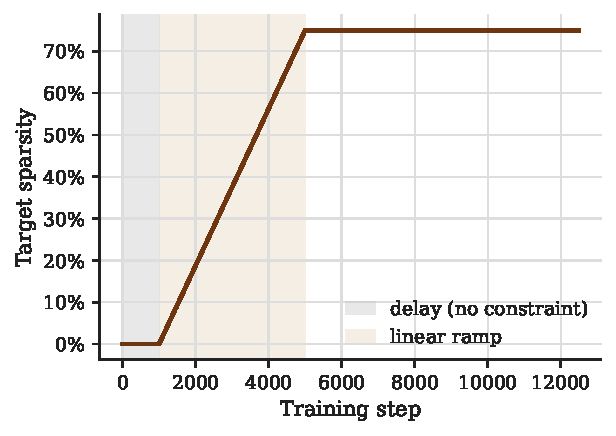
\includegraphics[width=\linewidth]{figures/figs/sparsity_rampup.pdf}
        \subcaption{Target sparsity schedule with the delay and linear ramp phases.}
        \label{fig:zon_rampup}
    \end{minipage}
    \hfill
    \begin{minipage}[t]{0.49\columnwidth}
        \centering
        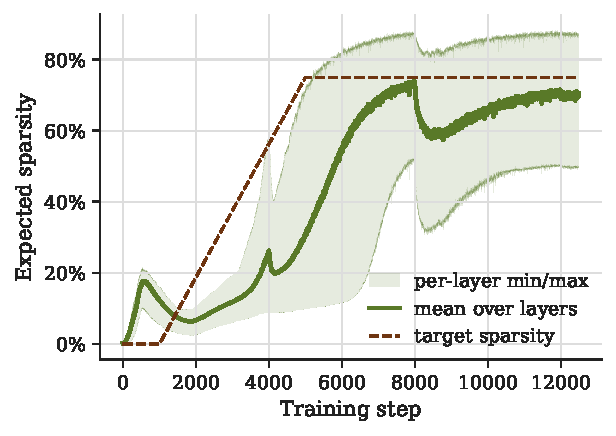
\includegraphics[width=\linewidth]{figures/figs/expected_sparsity.pdf}
        \subcaption{The convergence of the expected sparsity.}
        \label{fig:zon_expected_sparsity}
    \end{minipage}
    \caption{Training dynamics of the adaptive ZoN gate.}
    \label{fig:zon_training_dynamics}
\end{figure}

Table~\ref{tab:zon_benchmarks} shows that ZoN-1.2B-A600M reaches a CORE score of
29.77, compared with 29.61 for Dense-1.2B and 27.35 for Dense-600M.
ZoN therefore achieves similar aggregate performance to the larger dense model
while using roughly 600M active parameters per token. Compared with the dense
model of similar active size, it improves CORE by 2.42 percentage points.
This supports the idea that keeping a larger memory and selecting which parts
to activate in the interemediate dimension can be more effective than using a smaller dense memory.

The comparison with Dense-600M is consistent across many tasks. For example,
ZoN improves HellaSwag accuracy from 57.24\% to 61.24\%, CommonsenseQA from
21.38\% to 28.67\%, and QA Wikidata from 46.44\% to 50.51\%.
Compared with Dense-1.2B, ZoN performs better on
Winograd and SQuAD, but worse on PIQA, ARC-Challenge, and CommonsenseQA.
Hance, the small CORE difference of 0.16 percentage points between the dense and sparse
1.2B models reflects comparable overall performance rather than a 
consistent advantage over the larger dense model.

As described above, we gradually increase the target sparsity during training
to let the model focus on language modeling at the beginning.
Figure~\ref{fig:zon_rampup} shows this schedule, while
Figure~\ref{fig:zon_expected_sparsity} shows that the expected sparsity closely
follows it. This suggests that suitable sparse kernels could accelerate
training once sparsity emerges. For longer training runs, the same delay and
ramp would account for a smaller fraction of the total training steps.
The sparsity constraint applies to an average over input tokens, so individual
tokens and tasks can have different sparsity levels.
The reported sparsity of approximately 70\% is an average across evaluation tasks.
Table~\ref{tab:zon_tasks} reports the predicted sparsity (Zero frac.) for each
task, along with the centered accuracies used to compute the CORE metric.
\begin{table}[h]
\caption{Evaluation of the dense and ZoN sparse runs. All entries are percentages;
CORE is the mean centered score. $\%0$ measures the fraction of zero ZoN
MLP gates in the sparse run. BB denotes BIG-bench.}
\label{tab:zon_tasks}
\begin{center}
\small
\setlength{\tabcolsep}{4pt}
\begin{tabular}{lrrrrr}
\toprule
& \multicolumn{2}{c}{Accuracy} & \multicolumn{2}{c}{Centered} & Predicted $\%0$. \\
\cmidrule(lr){2-3}\cmidrule(lr){4-5}
Task & Dense & Sparse & Dense & Sparse & Sparse \\
\midrule
HellaSwag (zero-shot) & 61.79 & 60.52 & 49.05 & 47.35 & 69.19 \\
Jeopardy & 15.21 & 15.07 & 15.21 & 15.07 & 65.20 \\
BB: QA Wikidata & 51.30 & 50.51 & 51.30 & 50.51 & 65.30 \\
ARC-Easy & 72.10 & 70.67 & 62.79 & 60.89 & 69.56 \\
ARC-Challenge & 42.66 & 40.96 & 23.55 & 21.27 & 69.40 \\
COPA & 64.00 & 68.00 & 28.00 & 36.00 & 67.41 \\
CommonsenseQA & 32.02 & 28.67 & 15.03 & 10.83 & 71.84 \\
PIQA & 76.93 & 75.35 & 53.86 & 50.71 & 69.14 \\
OpenBookQA & 43.20 & 41.40 & 24.27 & 21.87 & 68.05 \\
LAMBADA (OpenAI) & 46.81 & 46.96 & 46.81 & 46.96 & 66.17 \\
HellaSwag & 62.05 & 61.24 & 49.40 & 48.32 & 68.29 \\
Winograd & 68.13 & 73.63 & 36.26 & 47.25 & 67.09 \\
WinoGrande & 60.30 & 60.77 & 20.60 & 21.55 & 66.98 \\
BB: Dyck languages & 13.10 & 11.60 & 13.10 & 11.60 & 75.95 \\
AGI Eval: LSAT-AR & 22.17 & 22.17 & 2.72 & 2.72 & 72.12 \\
BB: CS algorithms & 39.39 & 44.32 & 39.39 & 44.32 & 73.14 \\
BB: Operators & 17.62 & 19.05 & 17.62 & 19.05 & 73.53 \\
BB: Repeat copy logic & 0.00 & 0.00 & 0.00 & 0.00 & 70.89 \\
SQuAD & 46.34 & 48.20 & 46.34 & 48.20 & 67.87 \\
CoQA & 34.22 & 35.04 & 34.22 & 35.04 & 68.45 \\
BoolQ & 63.79 & 61.31 & 4.72 & -1.80 & 67.76 \\
BB: Language identification & 24.77 & 24.81 & 17.24 & 17.28 & 67.62 \\
\midrule
CORE & --- & --- & 29.6130 & 29.7722 & --- \\
\bottomrule
\end{tabular}
\end{center}
\end{table}


\section{Generalization to embedding language models}
\label{sec:embedding_models}

We apply the same principle to embedding language models, using ZoN to predict
which coordinates of an embedding to keep. Here, we use NV-Embed representations
and train the gates without a specific target sparsity constraint. Unlike the MLP setting, we
stretch on both the left and right sides and clip the gates to $[0,1]$, encouraging
gates to be either zero or one. This saves disk memory as for vector store, binary
gates are cheaper. At inference, we keep the $k$ coordinates with
the highest sigmoid gate scores, with $k\in\{128,256\}$ for evaluation,
but $k$ can be chosen freely during inferene, depending on the budget. 

\paragraph{Experimental setup.}
For retrieval, we train a linear projector of shape
$d_{\text{model}}\times d_{\text{model}}$ on top of the embeddings, alongside
the gate projector. For classification, we instead use two a perceptron,
with linear projectors $d_{\text{model}}$ to $4d_{\text{model}}$ and back to $d_{\text{model}}$,
with a ReLU activation between them. In both settings, the gate network uses
a hidden dimension of $r=d_{\text{model}} / 4$, with $d_{\text{model}}$ being
4096 for NV-Embed.
We evaluate retrieval on NFCorpus and SciFact using NDCG@10, and classification
on MTOPIntent and Banking77 using top-1 accuracy. We train for 10 epochs on
each dataset, except NFCorpus, where we use 2 epochs due to the training budget.

\begin{table}[t]
\centering
\caption{Performance of NV-Embed representations on classification and retrieval
tasks. Scores are percentages. $k$ is the number of coordinates retained at
inference; dense representations use all $d_{\text{model}}$ coordinates.
The dense baseline uses NV-Embed with a projector fine-tuned on each task
and retains all coordinates. The best score in each column is bold and the second-highest
distinct score is underlined.}
\label{tab:embedding_results}
\small
\setlength{\tabcolsep}{3pt}
\begin{tabular}{llc|cc|cc}
\toprule
& & & \multicolumn{2}{c|}{\textbf{Classification}} & \multicolumn{2}{c}{\textbf{Retrieval}} \\
& & & \multicolumn{2}{c|}{Top-1 Acc. (\%) $\uparrow$} & \multicolumn{2}{c}{NDCG@10 (\%) $\uparrow$} \\
\cmidrule{4-5}\cmidrule{6-7}
Category & Method & Dim. & MTOPIntent & Banking77 & NFCorpus & SciFact \\
\midrule
Dense & Fine-tuned & $d_{\text{model}}$ & \underline{93.96} & \underline{93.73} & 55.01 & \textbf{84.87} \\
\midrule
& CSR & 256 & \textbf{96.85} & \textbf{94.38} & \textbf{56.12} & 73.20 \\
& CSR & 128 & \textbf{96.85} & \textbf{94.38} & 54.64 & 73.20 \\
\cmidrule{2-7}
\rowcolor{ratioDenseD!40!white}
\cellcolor{white} & ZoN (ours) & 256 & 91.68 & 92.93 & \underline{55.46} & \underline{82.06} \\
\rowcolor{ratioDenseD!40!white}
\cellcolor{white}\multirow{-4}{*}{Sparse} & ZoN (ours) & 128 & 90.04 & 91.02 & 52.14 & 81.23 \\
\bottomrule
\end{tabular}
\end{table}


\paragraph{Results.}
Table~\ref{tab:embedding_results} shows that the benefit depends on the task.
On SciFact, ZoN outperforms CSR, but remains below the full
fine-tuned representation. On NFCorpus, ZoN with $k=256$ slightly exceeds
the full fine-tuned representation, while CSR is better overall.
For classification, ZoN remains below both CSR and the baseline using NV-Embed
with a projector fine-tuned on the task and all embedding coordinates retained.
Increasing $k$ from 128 to 256 improves ZoN on all four tasks.
These results suggest that adaptive coordinate selection can preserve much
of the retrieval performance.

\bibliography{iclr2027_conference}
\bibliographystyle{iclr2027_conference}

\appendix

\section{Appendix}
You may include other additional sections here.


\end{document}
